\documentclass[11pt]{article}
\usepackage{amsmath, amssymb, amsthm}
\usepackage{xcolor}
\usepackage[most]{tcolorbox}
\usepackage{geometry}
\geometry{margin=1.5cm}
\usepackage{graphicx}
\usepackage{enumitem}
\usepackage{tikz}
\usepackage{tikz-3dplot}
\usepackage{multicol}
\usepackage{lmodern}
\usepackage{setspace}
\usepackage{titlesec}
\usepackage{fancyhdr}
\usetikzlibrary{arrows.meta}
\usepackage{array}
\usepackage{booktabs}
\usepackage{hyperref}


\setlength{\parindent}{0pt}

\begin{document}

\begin{figure}[!ht]
    \centering
    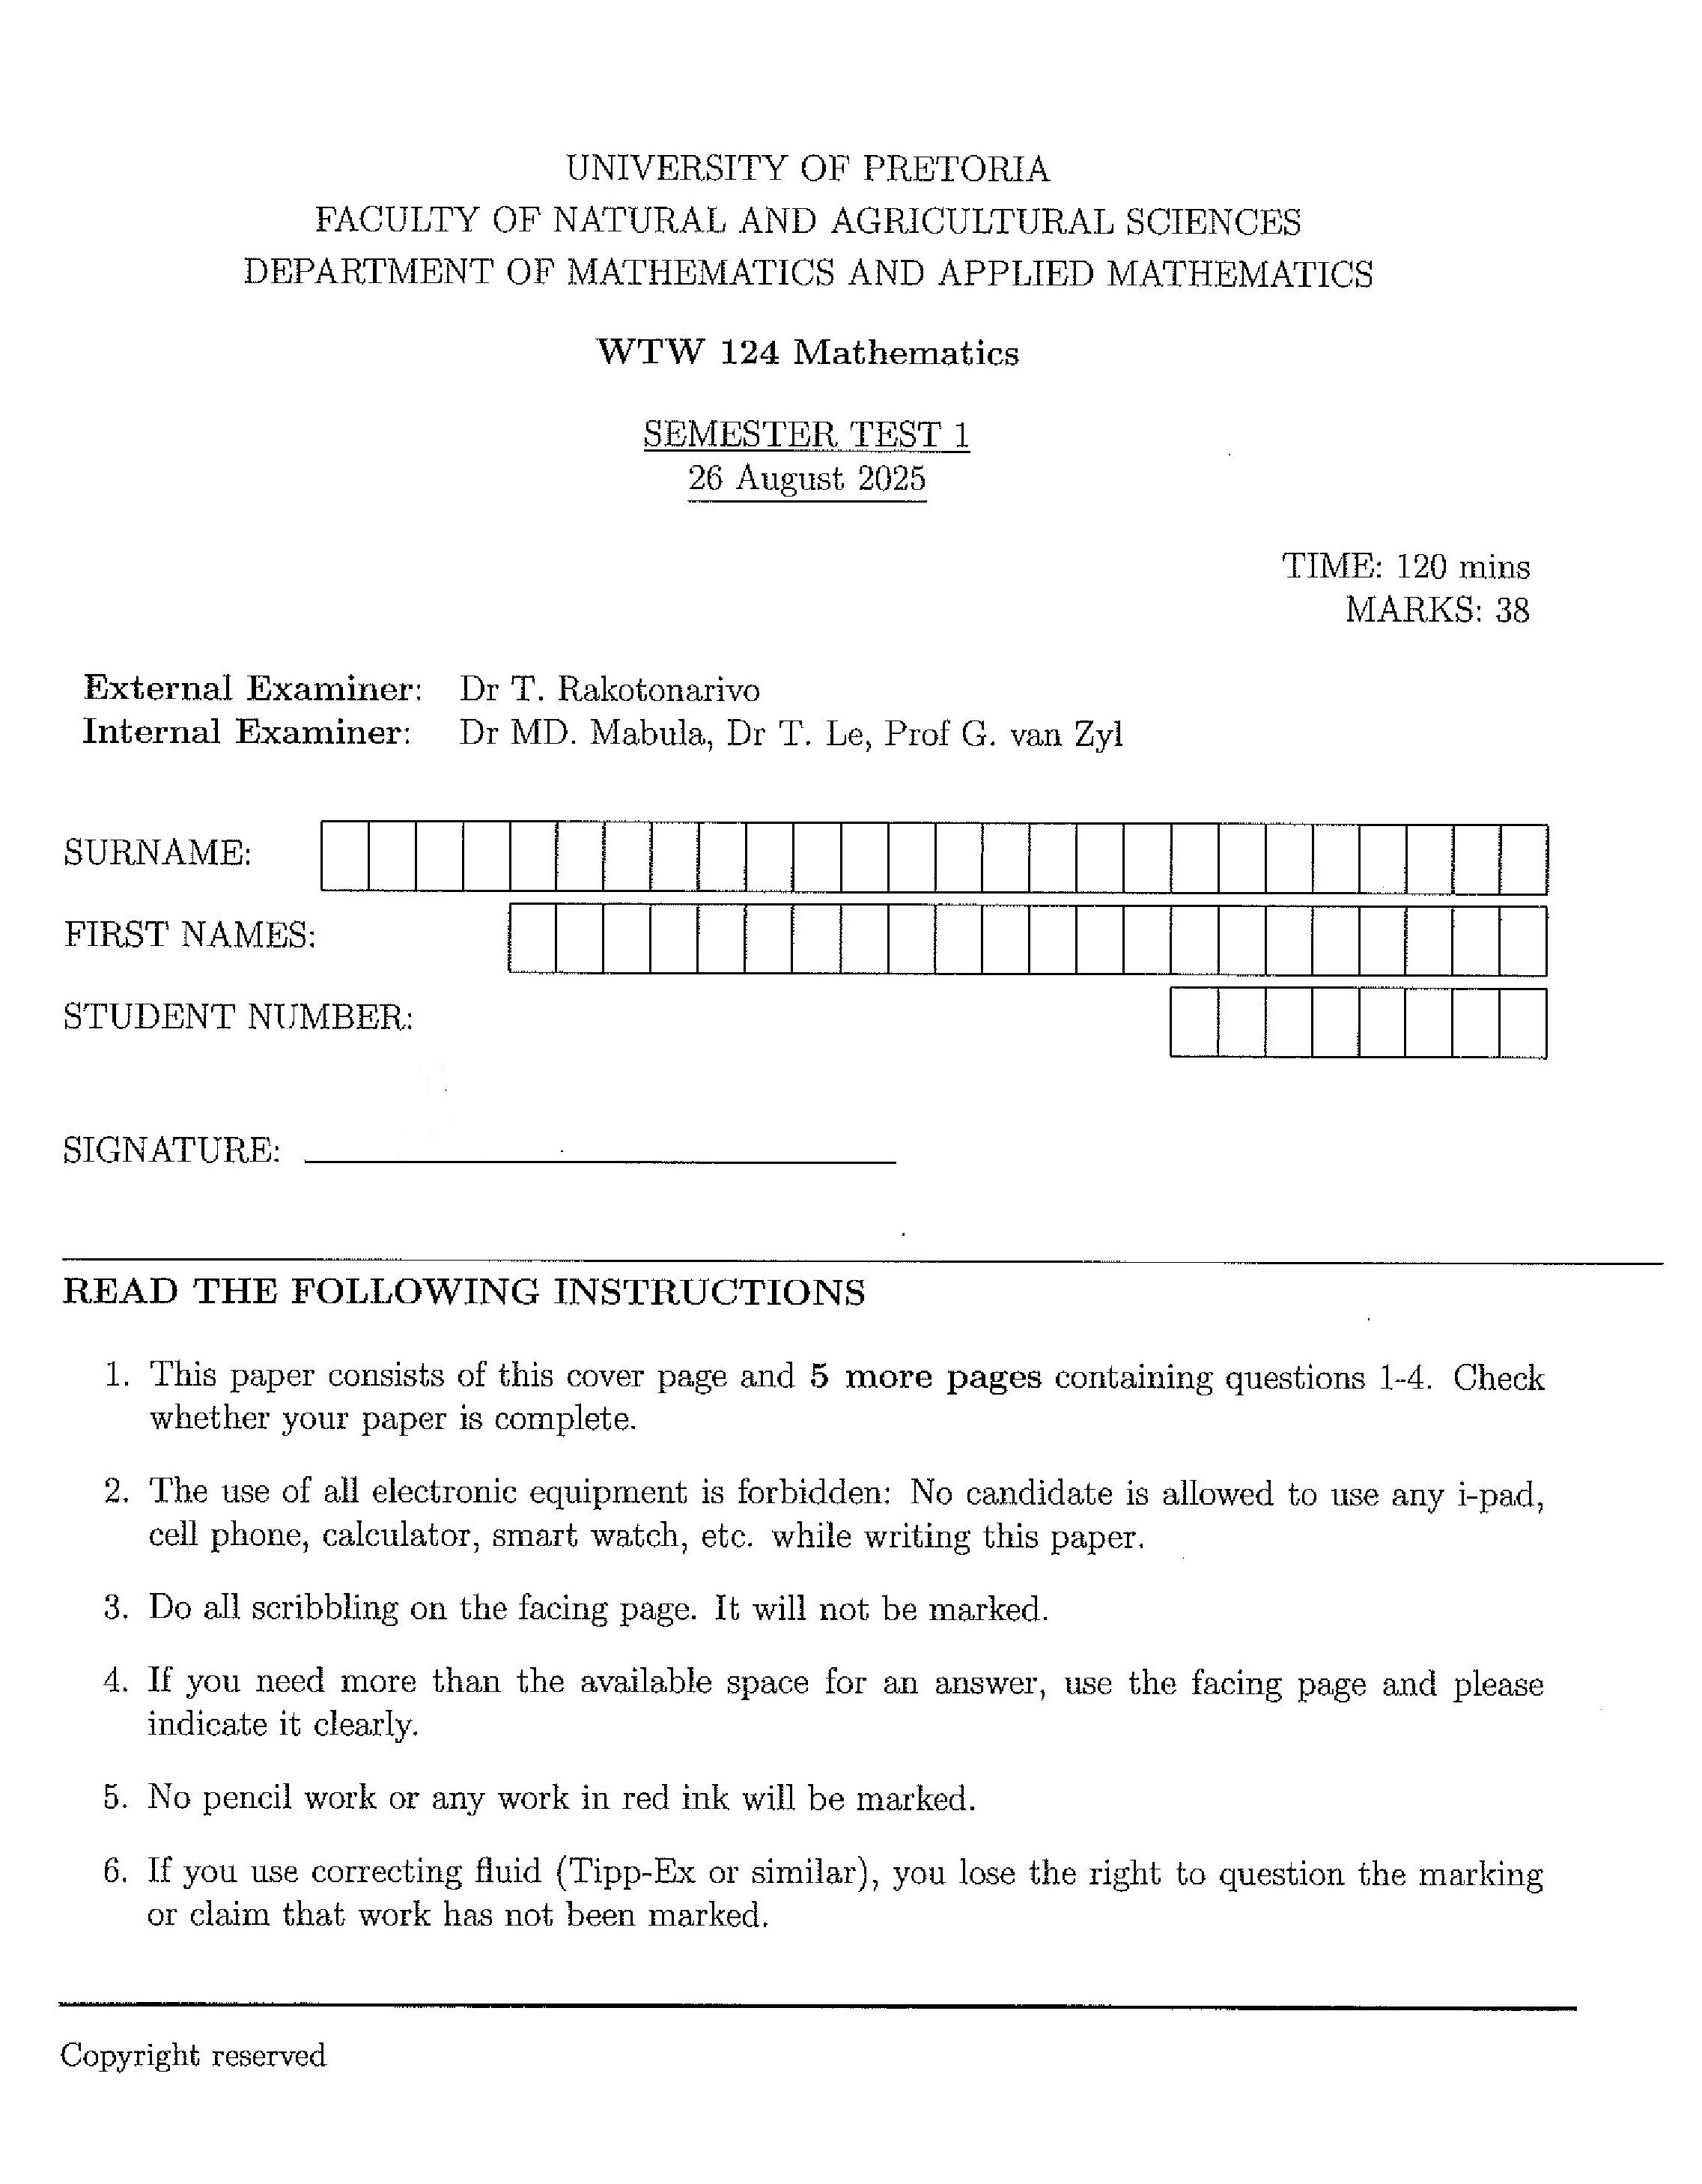
\includegraphics[width=1\textwidth]{TitleQP.jpg}
\end{figure}

\newpage

\textbf{Question 1.}
\begin{enumerate}[label=\alph*)]
    \item Find two unit vectors perpendicular to both vectors \(\bar{u} =\langle1,2,-1\rangle\) and \(\bar{v}=\langle3,1,2\rangle\). \hfill [3]
    \vspace{8cm}
    \item Let \(\bar{u}\) and \(\bar{v}\) be two non-zero vectors such that \(\bar{u} \cdot  \bar{v} = \|\bar{u} \times \bar{v}\|\).
    Find the magnitude of the angle between the rays determined by \(\bar{u}\) and \(\bar{v}\) \hfill [3]
    \vspace{8cm}
    \item Let \(A\), \(B\) and \(C\) be three matrices such that \(ABC\) exists, where \(A\) has size \(3\times3\) and \(C\) has size \(5\times5\).
    Describe the sizes \(B\) and \(ABC\). \hfill [2]
\end{enumerate}

\newpage

\textbf{Question 2.}
\begin{enumerate}[label=\alph*)]
    \item Let \(\bar{u}\) and \(\bar{v}\) be vectors in \(\mathbb{R}^3\). Prove that if \(\bar{u}+\bar{v} = \bar{0}\), then \(\bar{u}\times\bar{v} = \bar{0}\). \hfill [3]
    \vspace{8cm}
    \item Let \(A\) be a \(2\times2\) matrix. Prove or disprove the following statement: If \(A(A-I) = 0\), then \(A = 0 \text{ or } A = I\). \hfill [3]
    \vspace{8cm}
    \item Let \(A\) and \(B\) be \(n\times n\) matrices. Prove that if \(AB = BA\), then \(A^T\) commutes with \(B^T\). \hfill [3]
\end{enumerate}

\newpage

\textbf{Question 3.}
\begin{enumerate}[label=\alph*)]
    \item Use Gaussian elimination to find (if possible) conditions on real numbers \(a\) such that the following system of linear equations
    has no solution: \hfill [4]

    \[ x + ay - z = 1\]
    \[ -x + (a-2)y + z = -1\]
    \[ 2x + 2y + (a-2)z = 1\]
    \vspace{8cm}
    \item Consider the following matrices:
    \[
A = \begin{bmatrix}
1 & -2 & 2 \\
2 & 1 & 1 \\
1 & 0 & 1
\end{bmatrix}
\text{ and } 
B = \begin{bmatrix}
    1 & 2 & -4 \\
    -1 & -1 & 3 \\
    -1 & -2 & 5
\end{bmatrix}.
\]

Do \(A\) and \(B\) commute? Show all steps. \hfill [3]

\end{enumerate}

\newpage

\textbf{Question 4.}

Consider the following two lines in \(\mathbb{R}^3\):
    \[
        L_1 = \{\langle1,2,-3\rangle + t\langle1,2,-3\rangle : t \in \mathbb{R}\}
        \text{ and }
        L_2 = \{\langle-3,1,0\rangle + t\langle-2,4,-6\rangle : t \in \mathbb{R}\}.
    \]
\begin{enumerate}[label=\alph*), series=Last]
    \item If \(P\) is a plane with equation \(2x-y-z=3\), then \(L_1 \subseteq P\).\\
    Is this statement true or false? Explain with full details. \hfill [3]
    \vspace{8cm}
    \item Give Cartesian equations for two parallel, each containing one of the lines above. \hfill [4]
\end{enumerate}

\newpage

\begin{enumerate}[label=\alph*),resume=Last]
    \item Let \(L\) be a line passing through the point \(\bar{p} = \langle2,0,0\rangle\) such that \(L\) is
    perpendicular to the line \(L_2\) at their intersection. Find a vector equation of the line \(L\). \hfill [4]
    \vspace{10cm}
    \item Find the equation of the line through the point \(\bar{p} = \langle2,-1,4\rangle\) and perpendicular to the
    plane\\ \(3x-2y-z=0\). \hfill [3]
\end{enumerate}
\end{document}